\documentclass[../../main.tex]{subfiles}

\graphicspath{{../../image/}{../../figure/}}

\begin{document}

\section{Markov 链 Monte Carlo 采样}\label{section:ch14-mcmc}

在上一节中，我们讨论了用于计算函数期望的拒绝采样和重要性采样策略，并且我们看到它们在高维空间中有严重局限性。本节将讨论一种非常通用和强大的采样策略，称为 Markov 链 Monte Carlo（Markov chain Monte Carlo，MCMC）采样，它允许从多种分布中进行采样并且可以很好地扩展到高维样本空间。Markov 链 Monte Carlo 采样起源于物理学（Metropolis and Ulam, 1949），直至 20 世纪 80 年代末期才开始在统计学领域产生显著影响。

与拒绝采样和重要性采样一样，我们依然从提议分布中采样。然而这一次，我们保持当前状态 $\bm{z}^{(\tau)}$ 的记录，提议分布 $q\!\left(\bm{z}\mid\bm{z}^{(\tau)}\right)$ 以当前状态为条件，因此样本序列 $\bm{z}^{(1)},\bm{z}^{(2)},\cdots$ 形成一个 Markov 链（参见\cref{subsection:ch14-markov链}）。同样，尽管 $Z_{p}$ 的值可能是未知的，如果我们将 $p(\bm{z})$ 写成 $p(\bm{z})=\widetilde{p}(\bm{z})/Z_{p}$，我们假设对于任意给定的 $\bm{z}$ 值，$\widetilde{p}(\bm{z})$ 可以很容易计算出来。我们的提议分布足够简单，可以直接从中抽取样本。在算法的每一个迭代中，我们从提议分布中生成一个候选样本 $\bm{z}^{\star}$，然后根据一个适当的准则来接受该样本。

\subsection{Metropolis 算法}\label{subsection:ch14-Metropolis算法}

在基础的 Metropolis 算法（Metropolis et al., 1953）中，我们假设提议分布是对称的，即对于所有的 $\bm{z}_{A}$ 和 $\bm{z}_{B}$ 值，有 $q\!\left(\bm{z}_{A}\mid\bm{z}_{B}\right)=q\!\left(\bm{z}_{B}\mid\bm{z}_{A}\right)$。然后候选样本以如下概率被接受：
\begin{align}
A\!\left(\bm{z}^{\star},\bm{z}^{(\tau)}\right)=\min\left(1,\frac{\widetilde{p}\!\left(\bm{z}^{\star}\right)}{\widetilde{p}\!\left(\bm{z}^{(\tau)}\right)}\right),
\label{align:ch14-metropolis接受概率}
\end{align}
这可以通过选择一个在单位区间 $(0,1)$ 上均匀分布的随机数 $u$ 来实现：如果 $A\!\left(\bm{z}^{\star},\bm{z}^{(\tau)}\right)>u$，则接受该样本。请注意，如果从 $\bm{z}^{(\tau)}$ 到 $\bm{z}^{\star}$ 的步骤导致 $p(\bm{z})$ 的值增加，那么候选样本一定会被保留。

\begin{definition}[Metropolis 算法]\label{definition:ch14-Metropolis算法}
设目标分布为 $p(\bm{z})=\widetilde{p}(\bm{z})/Z_{p}$，$Z_{p}$ 未知，提议分布 $q$ 关于其两个自变量对称。Metropolis 算法按下述方式生成 Markov 链：给定当前状态 $\bm{z}^{(\tau)}$，从 $q\!\left(\bm{z}\mid\bm{z}^{(\tau)}\right)$ 中抽取候选样本 $\bm{z}^{\star}$，以\eqref{align:ch14-metropolis接受概率}给出的概率 $A\!\left(\bm{z}^{\star},\bm{z}^{(\tau)}\right)$ 接受它，并令
\begin{align*}
\bm{z}^{(\tau+1)}=\begin{cases}\bm{z}^{\star}, & \text{若接受},\\ \bm{z}^{(\tau)}, & \text{若拒绝}.\end{cases}
\end{align*}
\end{definition}

% SUPPLEMENT: parent=definition:ch14-Metropolis算法; kind=motivation; location=紧随其后的 remark（重构新增）
\begin{remark}（重构新增）Metropolis 算法用「按目标密度比决定去留」代替了拒绝采样中的比较函数：分子分母中的未知常数 $Z_{p}$ 自动相消，因此无需知道归一化常数，也无需寻找包络。对称性条件不可省：只有 $q\!\left(\bm{z}^{\star}\mid\bm{z}^{(\tau)}\right)=q\!\left(\bm{z}^{(\tau)}\mid\bm{z}^{\star}\right)$ 时，接受率才恰为 $\widetilde{p}(\bm{z}^{\star})/\widetilde{p}(\bm{z}^{(\tau)})$；否则必须补上提议分布之比，这就是\cref{subsection:ch14-Metropolis-Hastings}的推广。注意接受率取 $\min(1,\cdot)$：当候选状态的密度更高时总是接受，当密度更低时按比例接受，这一「有偏的爬山」正是让链停留在 $p$ 的高密度区而不至于永远卡在局部极大值的原因。最后，拒绝时链原地不动（$\bm{z}^{(\tau+1)}=\bm{z}^{(\tau)}$），样本序列中会出现重复值，这是 Metropolis 与拒绝采样的本质区别：被拒绝的信息被保留而非丢弃。
\end{remark}

下面给出 Metropolis 采样的完整流程。

\begin{quote}
\small
\textbf{算法 14.1：Metropolis 采样}\\
\textbf{输入：}未归一化分布 $\widetilde{p}(\bm{z})$；提议分布 $q\!\left(\bm{z}\mid\widetilde{\bm{z}}\right)$；初始状态 $\bm{z}^{(0)}$；迭代次数 $T$。\\
\textbf{输出：}$\bm{z}\sim\widetilde{p}(\bm{z})$。\\
$\bm{z}_{\mathrm{prev}}\leftarrow\bm{z}^{(0)}$；\\
对 $\tau\in\{1,\cdots,T\}$：\\
\quad 从提议分布中采样 $\bm{z}^{\star}\sim q\!\left(\bm{z}\mid\bm{z}_{\mathrm{prev}}\right)$；\\
\quad 从均匀分布中采样 $u\sim\mathcal{U}(0,1)$；\\
\quad 若 $\widetilde{p}\!\left(\bm{z}^{\star}\right)/\widetilde{p}\!\left(\bm{z}_{\mathrm{prev}}\right)>u$，则 $\bm{z}_{\mathrm{prev}}\leftarrow\bm{z}^{\star}$（即 $\bm{z}^{(\tau)}=\bm{z}^{\star}$）；否则保持 $\bm{z}_{\mathrm{prev}}$ 不变（即 $\bm{z}^{(\tau)}=\bm{z}^{(\tau-1)}$）；\\
返回 $\bm{z}_{\mathrm{prev}}$（即 $\bm{z}^{(T)}$）。
\end{quote}

如果候选样本被接受，则 $\bm{z}^{(\tau+1)}=\bm{z}^{\star}$，否则候选样本 $\bm{z}^{\star}$ 将被丢弃：将 $\bm{z}^{(\tau+1)}$ 设置为 $\bm{z}^{(\tau)}$，并从分布 $q\!\left(\bm{z}\mid\bm{z}^{(\tau+1)}\right)$ 中抽取另一个候选样本。这与拒绝采样形成了鲜明对比，在拒绝采样中，被拒绝的样本将直接被丢弃。在 Metropolis 算法中，当一个候选样本被拒绝时，它的前一个样本将包含在最终的样本列表中，导致样本有多个副本。当然，在实际应用中，每个保留的样本只会有一个副本，并附带一个整数权重因子，用于记录该状态出现的次数。

\begin{figure}[htbp]
\centering
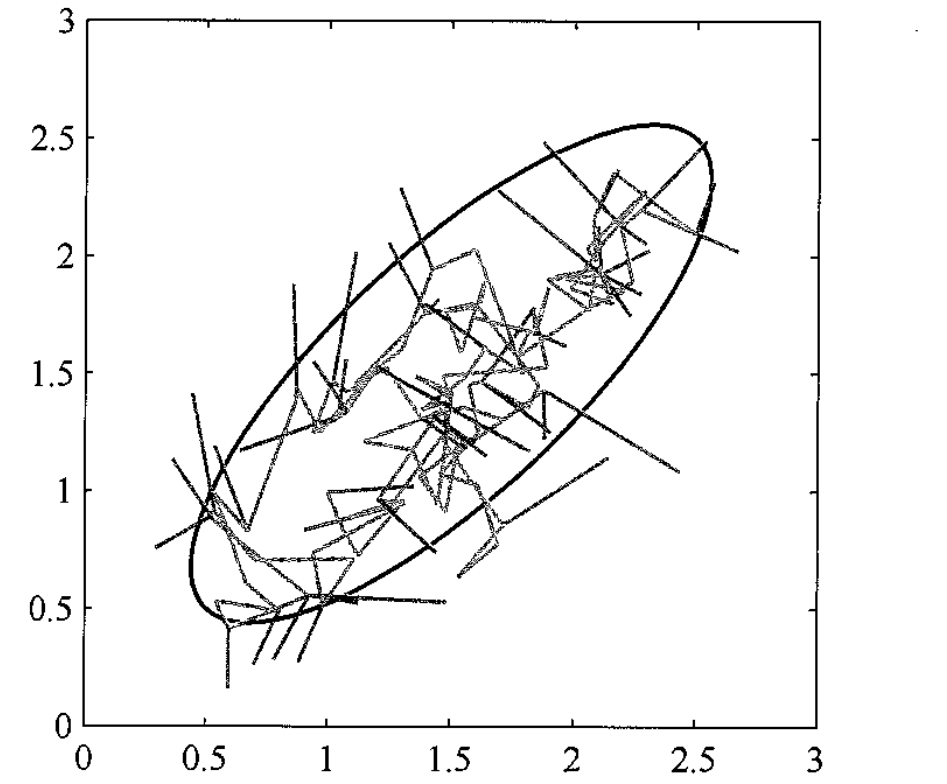
\includegraphics[width=0.42\textwidth]{ch14-fig14.9-metropolis-traj.png}
\caption{使用 Metropolis 算法从 Gauss 分布中采样的简单示意图，该 Gauss 分布的一个标准差等高线是用椭圆显示的。提议分布是一个各向同性的 Gauss 分布，其标准差为 $0.2$。接受的候选样本以绿线显示，拒绝的候选样本以红线显示。共生成 $150$ 个候选样本，其中 $43$ 个被拒绝}
\label{figure:ch14-metropolis轨迹}
\end{figure}

正如我们将看到的，如果对于任何的 $\bm{z}_{A}$ 和 $\bm{z}_{B}$ 值，$q\!\left(\bm{z}_{A}\mid\bm{z}_{B}\right)$ 都是正值（这是一个充分但非必要条件），则 $\bm{z}^{(\tau)}$ 的分布趋向于 $p(\bm{z})$（当 $\tau\rightarrow\infty$ 时）。然而，应该强调的是，序列 $\bm{z}^{(1)},\bm{z}^{(2)},\cdots$ 不是来自 $p(\bm{z})$ 的独立样本集，因为连续的样本高度相关。如果希望获得独立的样本，那么我们可以丢弃大部分序列，每次只保留第 $M$ 个样本。对于足够大的 $M$，保留的样本将在实际意义上是独立的。\cref{figure:ch14-metropolis轨迹}显示了一个简单的示例，它使用 Metropolis 算法从二维 Gauss 分布中进行采样，其中提议分布是各向同性的 Gauss 分布。

为了深入了解 Markov 链 Monte Carlo 采样算法的本质，我们观察一个具体例子（即随机游走）的性质。考虑一个由整数构成的状态空间 $\mathbb{Z}$，已知概率
\begin{align}
p\!\left(z^{(\tau+1)}=z^{(\tau)}\right)&=0.5,
\label{align:ch14-随机游走停留}\\
p\!\left(z^{(\tau+1)}=z^{(\tau)}+1\right)&=0.25,
\label{align:ch14-随机游走右移}\\
p\!\left(z^{(\tau+1)}=z^{(\tau)}-1\right)&=0.25,
\label{align:ch14-随机游走左移}
\end{align}
其中 $z^{(\tau)}$ 表示在时间步 $\tau$ 的状态。

\begin{example}[ 整数上的简单随机游走]\label{example:ch14-随机游走}
设 $\left\{z^{(\tau)}\right\}$ 按\eqref{align:ch14-随机游走停留}～\eqref{align:ch14-随机游走左移}演化，初始状态 $z^{(0)}=0$。求 $\mathbb{E}\left[z^{(\tau)}\right]$ 与 $\mathbb{E}\left[\left(z^{(\tau)}\right)^{2}\right]$。
\end{example}

\begin{solution}（重构新增）由对称性，给定 $z^{(\tau-1)}=z$ 时，
\begin{align*}
\mathbb{E}\left[z^{(\tau)}\mid z^{(\tau-1)}=z\right]=0.5z+0.25(z+1)+0.25(z-1)=z,
\end{align*}
故 $\mathbb{E}\left[z^{(\tau)}\right]=\mathbb{E}\left[z^{(\tau-1)}\right]=\cdots=z^{(0)}=0$。又
\begin{align*}
\mathbb{E}\left[\left(z^{(\tau)}\right)^{2}\mid z^{(\tau-1)}=z\right]=0.5z^{2}+0.25(z+1)^{2}+0.25(z-1)^{2}=z^{2}+\frac{1}{2},
\end{align*}
故 $\mathbb{E}\left[\left(z^{(\tau)}\right)^{2}\right]=\mathbb{E}\left[\left(z^{(\tau-1)}\right)^{2}\right]+\frac{1}{2}$，归纳得 $\mathbb{E}\left[\left(z^{(\tau)}\right)^{2}\right]=\tau/2$（见\cref{exercise:ch14-11}）。
\end{solution}

因此，在时间步 $\tau$ 之后，随机游走平均而言仅行进了与 $\sqrt{\tau}$ 成比例的距离。这种平方根依赖性是随机游走行为的典型特征，表明随机游走在探索状态空间时效率非常低。正如我们将看到的，设计 Markov 链 Monte Carlo 采样算法的一个核心目标就是避免随机游走行为。

\subsection{Markov 链}\label{subsection:ch14-markov链}

在更详细地讨论 Markov 链 Monte Carlo 采样之前，我们先研究一下 Markov 链的一般性质。特别地，我们想知道 Markov 链在何种情况下会收敛到期望的分布。

\begin{definition}[一阶 Markov 链]\label{definition:ch14-markov链}
称随机变量序列 $\bm{z}^{(1)},\cdots,\bm{z}^{(M)}$ 为一阶 Markov 链，若对每个 $m\in\{1,\cdots,M-1\}$ 都有条件独立性
\begin{align}
p\!\left(\bm{z}^{(m+1)}\mid\bm{z}^{(1)},\cdots,\bm{z}^{(m)}\right)=p\!\left(\bm{z}^{(m+1)}\mid\bm{z}^{(m)}\right).
\label{align:ch14-markov性}
\end{align}
\end{definition}

% SUPPLEMENT: parent=definition:ch14-markov链; kind=motivation; location=紧随其后的 remark（重构新增）
\begin{remark}（重构新增）\eqref{align:ch14-markov性}的含义是「给定现在，未来与过去条件独立」：链在时刻 $m+1$ 的状态只通过当前状态 $m$ 依赖历史，因此整条链的联合分布可由初始分布 $p\!\left(\bm{z}^{(1)}\right)$ 与转移核 $T_{m}$ 完全确定。这一「无记忆性」正是 MCMC 能够只用当前状态就生成下一个样本的原因，也是它相比拒绝采样、重要性采样能在高维工作而不需要全局包络的根本原因。一阶性是建模选择而非数学必然：二阶链需要保留两个历史状态，状态空间随之增大；本书只处理一阶链。
\end{remark}

这可以用一个链式的有向图模型来表示（见\cref{figure:ch11-离散节点链}）。然后，我们可以通过给出初始变量的概率分布 $p\!\left(\bm{z}^{(0)}\right)$ 和以转移概率（transition probabilities）形式表达的后续变量条件分布 $T_{m}\!\left(\bm{z}^{(m)},\bm{z}^{(m+1)}\right)\equiv p\!\left(\bm{z}^{(m+1)}\mid\bm{z}^{(m)}\right)$，即可完整定义 Markov 链。

\begin{definition}[齐次 Markov 链]\label{definition:ch14-齐次markov链}
若\cref{definition:ch14-markov链}中的转移概率 $T_{m}$ 对一切 $m$ 都相同，则称该 Markov 链是齐次的或同质（homogeneous）的，此时记 $T\!\left(\bm{z},\bm{z}'\right)=p\!\left(\bm{z}'\mid\bm{z}\right)$。
\end{definition}

% SUPPLEMENT: parent=definition:ch14-齐次markov链; kind=motivation; location=紧随其后的 remark（重构新增）
\begin{remark}（重构新增）齐次性把「随时刻变化的转移规则」简化为单个转移核 $T$，于是链的分布演化只依赖于 $T$ 的幂次，不变分布与遍历性的讨论才成为可能。本章构造的 MCMC 算法（Metropolis、Metropolis-Hastings、Gibbs）全部是齐次链，转移核不随 $\tau$ 改变；变分推断中使用的「退火」或「自适应」方案则会破坏齐次性，此时收敛性需要另行论证（例如 Robbins-Monro 型的学习率条件）。注意定义只要求条件分布相同，并不要求初始分布与 $T$ 有任何关系——初始分布只影响链的暂态，这正是 MCMC 需要 burn-in 的原因。
\end{remark}

链中的某个特定变量的边缘概率可以用 Markov 链中前一个变量的边缘概率表示为
\begin{align}
p\!\left(\bm{z}^{(m+1)}\right)=\int p\!\left(\bm{z}^{(m+1)}\mid\bm{z}^{(m)}\right)p\!\left(\bm{z}^{(m)}\right)\mathrm{d}\bm{z}^{(m)},
\label{align:ch14-链边缘}
\end{align}
其中的积分对于离散变量来说可以替换为求和。

\begin{definition}[不变分布]\label{definition:ch14-不变分布}
若分布 $p^{\star}(\bm{z})$ 满足
\begin{align}
p^{\star}(\bm{z})=\int T\!\left(\bm{z}',\bm{z}\right)p^{\star}\!\left(\bm{z}'\right)\mathrm{d}\bm{z}',
\label{align:ch14-不变分布}
\end{align}
则称 $p^{\star}$ 对该 Markov 链是不变的，也称 $p^{\star}$ 是平稳分布（stationary distribution）。若一个分布在 Markov 链的每个步骤都保持该分布不变，那么该分布对于这个 Markov 链来说就是不变的或者说稳定的。
\end{definition}

% SUPPLEMENT: parent=definition:ch14-不变分布; kind=motivation; location=紧随其后的 remark（重构新增）
\begin{remark}（重构新增）不变分布是 MCMC 的「目标」：只要目标分布 $p$ 对转移核不变，链一旦进入 $p$ 就会永远保持 $p$，因此用链上的样本估计 $p$ 下的期望才有意义。\eqref{align:ch14-不变分布}是一个泛函不动点方程，它并不保证 $p^{\star}$ 唯一：若转移概率由恒等变换给出，则任何分布都是不变的。所以「构造一个以 $p$ 为不变分布的链」只是第一步，还需要\cref{definition:ch14-遍历性}保证从任意初始分布出发都收敛到同一个 $p^{\star}$。对离散状态空间，\eqref{align:ch14-不变分布}就是 $p^{\star}=p^{\star}T$，即 $p^{\star}$ 是转移矩阵的左特征向量（特征值 $1$）。
\end{remark}

请注意，给定的 Markov 链可能有多个不变分布。例如，如果转移概率由恒等变换给出，那么任何分布都将是不变的。

\begin{definition}[详细平衡]\label{definition:ch14-详细平衡}
若转移概率 $T$ 与分布 $p^{\star}$ 满足
\begin{align}
p^{\star}(\bm{z})\,T\!\left(\bm{z},\bm{z}'\right)=p^{\star}\!\left(\bm{z}'\right)T\!\left(\bm{z}',\bm{z}\right),
\label{align:ch14-细致平衡}
\end{align}
则称它们满足详细平衡（detailed balance）性质。满足详细平衡性质的 Markov 链被称为可逆的（reversible）。
\end{definition}

% SUPPLEMENT: parent=definition:ch14-详细平衡; kind=motivation; location=紧随其后的 remark（重构新增）
\begin{remark}（重构新增）详细平衡比不变性更强：它要求每一对状态之间的「双向流量」逐点相等，而不只是总流量相等。验证详细平衡通常比直接验证\eqref{align:ch14-不变分布}容易得多，因为后者需要对整个状态空间积分，而前者只需比较两个密度的乘积；本章所有 MCMC 算法都是通过构造满足\eqref{align:ch14-细致平衡}的转移核来证明其正确性的。可逆性一词来自如下事实：在平稳状态下，正向轨迹 $\left(\bm{z}^{(1)},\bm{z}^{(2)},\cdots\right)$ 与反向轨迹的联合分布相同，即链在时间反演下统计等价。注意详细平衡是充分而非必要条件：存在不可逆的链（例如循环式的 Gibbs 扫描）仍以 $p$ 为不变分布。
\end{remark}

确保目标分布 $p(\bm{z})$ 是不变的一个充分（但非必要）条件是选择满足详细平衡性质的转移概率。对于特定的分布 $p^{\star}(\bm{z})$，容易看出，如果转移概率满足关于该分布的详细平衡性质，则保持该分布不变，因为
\begin{align}
\int p^{\star}\!\left(\bm{z}'\right)T\!\left(\bm{z}',\bm{z}\right)\mathrm{d}\bm{z}'&=\int p^{\star}(\bm{z})\,T\!\left(\bm{z},\bm{z}'\right)\mathrm{d}\bm{z}'\nonumber\\
&=p^{\star}(\bm{z})\int p\!\left(\bm{z}'\mid\bm{z}\right)\mathrm{d}\bm{z}'\nonumber\\
&=p^{\star}(\bm{z}).
\label{align:ch14-细致平衡推导}
\end{align}

\begin{proposition}[详细平衡蕴含不变性]\label{proposition:ch14-细致平衡蕴含不变}
设转移核 $T$ 与分布 $p^{\star}$ 满足\eqref{align:ch14-细致平衡}，且 $T\!\left(\bm{z},\cdot\right)$ 对每个 $\bm{z}$ 都是概率密度。则 $p^{\star}$ 是 $T$ 的不变分布，即\eqref{align:ch14-不变分布}成立。
\end{proposition}

\begin{proof}
由\eqref{align:ch14-细致平衡}，对任意 $\bm{z}$，
\begin{align*}
\int p^{\star}\!\left(\bm{z}'\right)T\!\left(\bm{z}',\bm{z}\right)\mathrm{d}\bm{z}'=\int p^{\star}(\bm{z})T\!\left(\bm{z},\bm{z}'\right)\mathrm{d}\bm{z}'=p^{\star}(\bm{z})\int T\!\left(\bm{z},\bm{z}'\right)\mathrm{d}\bm{z}'=p^{\star}(\bm{z}),
\end{align*}
最后一步用到 $T\!\left(\bm{z},\cdot\right)$ 是概率密度，即 $\int T\!\left(\bm{z},\bm{z}'\right)\mathrm{d}\bm{z}'=1$。这正是\eqref{align:ch14-不变分布}。
\end{proof}

% SUPPLEMENT: parent=proposition:ch14-细致平衡蕴含不变; kind=motivation; location=紧随其后的 remark（重构新增）
\begin{remark}（重构新增）证明只做了一次「换元 + 提公因子」，关键是把对 $\bm{z}'$ 的积分换成对 $\bm{z}'$ 的另一个方向的积分，从而把 $p^{\star}(\bm{z})$ 提到积分号外。条件「$T\!\left(\bm{z},\cdot\right)$ 是概率密度」不可省：若 $T$ 只是次随机核（例如 Metropolis 中遗漏了「拒绝时原地不动」这一项），则 $\int T\,\mathrm{d}\bm{z}'<1$，上式给出的是 $p^{\star}$ 被衰减而不是保持不变。这解释了算法描述中为何必须显式写出「拒绝则 $\bm{z}^{(\tau+1)}=\bm{z}^{(\tau)}$」：正是这一项补齐了转移核的概率质量，使\eqref{align:ch14-细致平衡推导}的归一化成立。
\end{remark}

我们的目标是使用 Markov 链从给定分布中采样。如果能建立一个 Markov 链使得目标分布是不变的，就可以达到目的。然而，我们还必须要求不管初始分布 $p\!\left(\bm{z}^{(0)}\right)$ 的选择如何，当 $m\rightarrow\infty$ 时，分布 $p\!\left(\bm{z}^{(m)}\right)$ 都收敛到所需的不变分布 $p^{\star}(\bm{z})$。

\begin{definition}[遍历性]\label{definition:ch14-遍历性}
若对任意初始分布 $p\!\left(\bm{z}^{(0)}\right)$，当 $m\rightarrow\infty$ 时 $p\!\left(\bm{z}^{(m)}\right)$ 都收敛到同一个不变分布 $p^{\star}(\bm{z})$，则称该 Markov 链是遍历的（ergodic），并称 $p^{\star}$ 为平衡（equilibrium）分布。
\end{definition}

% SUPPLEMENT: parent=definition:ch14-遍历性; kind=motivation; location=紧随其后的 remark（重构新增）
\begin{remark}（重构新增）遍历性是「无论从哪里出发都能到达并停留在 $p^{\star}$」的保证，它是 MCMC 可用性的另一半：不变性只保证「到了就不走」，遍历性才保证「一定会到」。显然一个遍历的 Markov 链只能有一个平衡分布。可以证明，一个齐次 Markov 链是遍历的，只需要对不变分布和转移概率施加较弱的约束条件（Neal, 1993），例如不可约（任意两个正概率区域互相可达）与非周期（不会按固定周期振荡）；这两个条件合起来保证 $T^{m}$ 收敛到秩一投影。实践中的主要障碍是不可约性：若目标分布有多个被零概率区域隔开的模态，而提议分布无法跨越这些区域，链就会被困在某个模态内，此时不变性依然成立但遍历性失效（见\cref{exercise:ch14-13}）。
\end{remark}

在实践中，我们经常利用一组「基础」转移 $B_{1},\cdots,B_{K}$ 来构造转移概率。这可以通过混合分布的形式来实现：
\begin{align}
T\!\left(\bm{z}',\bm{z}\right)=\sum_{k=1}^{K}\alpha_{k}B_{k}\!\left(\bm{z}',\bm{z}\right),
\label{align:ch14-混合转移}
\end{align}
混合系数 $\alpha_{1},\cdots,\alpha_{K}$ 必须满足 $\alpha_{k}\geqslant 0$ 且 $\sum_{k}\alpha_{k}=1$。「基础」转移可以通过连续应用结合起来，于是有
\begin{align}
T\!\left(\bm{z}',\bm{z}\right)=\sum_{z_{1}}\cdots\sum_{z_{K-1}}B_{1}\!\left(\bm{z}',\bm{z}_{1}\right)\cdots B_{K-1}\!\left(\bm{z}_{K-2},\bm{z}_{K-1}\right)B_{K}\!\left(\bm{z}_{K-1},\bm{z}\right).
\label{align:ch14-复合转移}
\end{align}

如果一个分布对每个基础转移都是不变的，那么很明显它也会对\eqref{align:ch14-混合转移}或\eqref{align:ch14-复合转移}给出的 $T\!\left(\bm{z}',\bm{z}\right)$ 保持不变。对于混合分布\eqref{align:ch14-混合转移}，如果每个基础转移都满足详细平衡条件，那么复合转移概率 $T$ 也将满足详细平衡条件。这对于使用\eqref{align:ch14-复合转移}构造的转移概率并不成立，尽管通过对基础转移的应用顺序进行对称化（即 $B_{1},B_{2},\cdots,B_{K},B_{K},\cdots,B_{2},B_{1}$），可以恢复详细平衡。使用复合转移概率的一个常见例子是让每个基础转移仅改变变量的一个子集。

\begin{proposition}[混合转移保持不变性]\label{proposition:ch14-混合转移不变}
设 $p^{\star}$ 对每个基础转移 $B_{k}$ 都不变，$\alpha_{k}\geqslant0$，$\sum_{k}\alpha_{k}=1$。则由\eqref{align:ch14-混合转移}定义的 $T$ 也不变 $p^{\star}$。若进一步每个 $B_{k}$ 都满足关于 $p^{\star}$ 的详细平衡，则 $T$ 也满足详细平衡。
\end{proposition}

\begin{proof}
由线性性，
\begin{align*}
\int T\!\left(\bm{z}',\bm{z}\right)p^{\star}\!\left(\bm{z}'\right)\mathrm{d}\bm{z}'=\sum_{k=1}^{K}\alpha_{k}\int B_{k}\!\left(\bm{z}',\bm{z}\right)p^{\star}\!\left(\bm{z}'\right)\mathrm{d}\bm{z}'=\sum_{k=1}^{K}\alpha_{k}p^{\star}(\bm{z})=p^{\star}(\bm{z}),
\end{align*}
即 $T$ 不变 $p^{\star}$。若每个 $B_{k}$ 满足详细平衡，则对每个 $k$ 有 $p^{\star}(\bm{z})B_{k}\!\left(\bm{z},\bm{z}'\right)=p^{\star}\!\left(\bm{z}'\right)B_{k}\!\left(\bm{z}',\bm{z}\right)$，两边乘 $\alpha_{k}$ 并对 $k$ 求和即得 $p^{\star}(\bm{z})T\!\left(\bm{z},\bm{z}'\right)=p^{\star}\!\left(\bm{z}'\right)T\!\left(\bm{z}',\bm{z}\right)$。
\end{proof}

% SUPPLEMENT: parent=proposition:ch14-混合转移不变; kind=motivation; location=紧随其后的 remark（重构新增）
\begin{remark}（重构新增）混合的直观含义是「每一步随机挑选一种更新方式」，因此只要每种方式都不破坏 $p^{\star}$，混合起来也不破坏；这是 Metropolis-Hastings 中「在不同提议分布之间轮换」以及 Gibbs 采样中「随机挑选一个变量更新」的理论依据。复合转移（连续应用）只保证不变性，不保证可逆性：两个各自可逆的核复合后一般不可逆，因为正向与反向的复合顺序相反；要对 $B_{1},\cdots,B_{K}$ 的复合恢复详细平衡，必须按 $B_{1},\cdots,B_{K},B_{K},\cdots,B_{1}$ 的顺序对称地应用。由于不变性已足以保证正确性，多数算法并不追求可逆性，但可逆性在证明收敛速度与构造控制变量时仍有用。
\end{remark}

\subsection{Metropolis-Hastings 算法}\label{subsection:ch14-Metropolis-Hastings}

前面我们介绍了基础的 Metropolis 算法，但没有实践证明它能从所需分布中进行采样。在给出证明之前，我们首先讨论一种更泛化的形式，称为 Metropolis-Hastings 算法（Hastings, 1970），该算法适用于提议分布不再是其参数的对称函数的情况。特别是在算法的第 $\tau$ 步，当前状态为 $\bm{z}^{(\tau)}$，首先从分布 $q_{k}\!\left(\bm{z}\mid\bm{z}^{(\tau)}\right)$ 中抽取一个样本 $\bm{z}^{\star}$，然后以概率 $A_{k}\!\left(\bm{z}^{\star},\bm{z}^{(\tau)}\right)$ 接受它，其中
\begin{align}
A_{k}\!\left(\bm{z}^{\star},\bm{z}^{(\tau)}\right)=\min\left(1,\frac{\widetilde{p}\!\left(\bm{z}^{\star}\right)q_{k}\!\left(\bm{z}^{(\tau)}\mid\bm{z}^{\star}\right)}{\widetilde{p}\!\left(\bm{z}^{(\tau)}\right)q_{k}\!\left(\bm{z}^{\star}\mid\bm{z}^{(\tau)}\right)}\right),
\label{align:ch14-mh接受概率}
\end{align}
这里的 $k$ 标记了正在考虑的可能转换集合的成员。同样，计算接受准则不需要知道概率分布 $p(\bm{z})=\widetilde{p}(\bm{z})/Z_{p}$ 中的归一化常数 $Z_{p}$。对于对称的提议分布，Metropolis-Hastings 准则\eqref{align:ch14-mh接受概率}可简化为标准的 Metropolis 准则\eqref{align:ch14-metropolis接受概率}。

\begin{definition}[Metropolis-Hastings 算法]\label{definition:ch14-Metropolis-Hastings算法}
给定未归一化目标分布 $\widetilde{p}$、一组提议分布 $\left\{q_{k}\right\}_{k=1}^{K}$ 以及迭代到分布下标的映射 $M(\cdot)$，Metropolis-Hastings 算法在第 $\tau$ 步取 $k=M(\tau)$，从 $q_{k}\!\left(\bm{z}\mid\bm{z}^{(\tau)}\right)$ 中抽取 $\bm{z}^{\star}$，以\eqref{align:ch14-mh接受概率}的概率接受它，拒绝时令 $\bm{z}^{(\tau+1)}=\bm{z}^{(\tau)}$。
\end{definition}

% SUPPLEMENT: parent=definition:ch14-Metropolis-Hastings算法; kind=motivation; location=紧随其后的 remark（重构新增）
\begin{remark}（重构新增）Metropolis-Hastings 相对 Metropolis 的唯一改动是接受率中多了一个提议分布之比 $q_{k}\!\left(\bm{z}^{(\tau)}\mid\bm{z}^{\star}\right)/q_{k}\!\left(\bm{z}^{\star}\mid\bm{z}^{(\tau)}\right)$。这一项的来源是：若提议分布偏向于某些方向（例如向高密度区偏移），则链会过度访问这些方向，必须用「返回概率」把偏差校正回来。它使算法对\emph{任意}提议分布都成立，因而允许使用梯度信息（如 Langevin 提议）或依赖当前状态的局部近似（如自适应拒绝采样），这是 Metropolis-Hastings 成为通用框架的原因。条件仍然只是 $q_{k}\!\left(\bm{z}^{\star}\mid\bm{z}^{(\tau)}\right)>0$ 当 $\widetilde{p}\!\left(\bm{z}^{\star}\right)>0$，以保证支撑集覆盖；归一化常数 $Z_{p}$ 依旧相消。
\end{remark}

\begin{quote}
\small
\textbf{算法 14.2：Metropolis-Hastings 采样}\\
\textbf{输入：}未归一化分布 $\widetilde{p}(\bm{z})$；提议分布 $\left\{q_{k}\!\left(\bm{z}\mid\bm{z}\right):k\in\{1,\cdots,K\}\right\}$；迭代下标到分布下标的映射 $M(\cdot)$；初始状态 $\bm{z}^{(0)}$；迭代次数 $T$。\\
\textbf{输出：}$\bm{z}\sim\widetilde{p}(\bm{z})$。\\
$\bm{z}_{\mathrm{prev}}\leftarrow\bm{z}^{(0)}$；\\
对 $\tau\in\{1,\cdots,T\}$：\\
\quad $k\leftarrow M(\tau)$；\\
\quad $\bm{z}^{\star}\sim q_{k}\!\left(\bm{z}\mid\bm{z}_{\mathrm{prev}}\right)$；\\
\quad $u\sim\mathcal{U}(0,1)$；\\
\quad 若 $\widetilde{p}\!\left(\bm{z}^{\star}\right)q_{k}\!\left(\bm{z}_{\mathrm{prev}}\mid\bm{z}^{\star}\right)/\left[\widetilde{p}\!\left(\bm{z}_{\mathrm{prev}}\right)q_{k}\!\left(\bm{z}^{\star}\mid\bm{z}_{\mathrm{prev}}\right)\right]>u$，则 $\bm{z}_{\mathrm{prev}}\leftarrow\bm{z}^{\star}$；否则保持不变；\\
返回 $\bm{z}_{\mathrm{prev}}$（即 $\bm{z}^{(T)}$）。
\end{quote}

我们可以通过证明\eqref{align:ch14-细致平衡}定义的详细平衡条件得以满足，从而进一步证明 $p(\bm{z})$ 是由 Metropolis-Hastings 算法所定义的 Markov 链的不变分布。利用\eqref{align:ch14-mh接受概率}，我们有
\begin{align}
p(\bm{z})\,q_{k}\!\left(\bm{z}'\mid\bm{z}\right)A_{k}\!\left(\bm{z},\bm{z}'\right)&=\min\left(p(\bm{z})q_{k}\!\left(\bm{z}'\mid\bm{z}\right),\,p\!\left(\bm{z}'\right)q_{k}\!\left(\bm{z}\mid\bm{z}'\right)\right)\nonumber\\
&=\min\left(p\!\left(\bm{z}'\right)q_{k}\!\left(\bm{z}\mid\bm{z}'\right),\,p(\bm{z})q_{k}\!\left(\bm{z}'\mid\bm{z}\right)\right)\nonumber\\
&=p\!\left(\bm{z}'\right)q_{k}\!\left(\bm{z}\mid\bm{z}'\right)A_{k}\!\left(\bm{z}',\bm{z}\right).
\label{align:ch14-mh细致平衡}
\end{align}
这个表达式在交换 $\bm{z}$ 和 $\bm{z}^{\star}$ 时是对称的，因此详细平衡成立。

\begin{proposition}[Metropolis-Hastings 的细致平衡]\label{proposition:ch14-mh细致平衡}
设 $p(\bm{z})=\widetilde{p}(\bm{z})/Z_{p}$，转移核为「以 $q_{k}$ 提议、以\eqref{align:ch14-mh接受概率}接受，拒绝时原地不动」，并记 $T_{k}\!\left(\bm{z},\bm{z}'\right)=q_{k}\!\left(\bm{z}'\mid\bm{z}\right)A_{k}\!\left(\bm{z},\bm{z}'\right)$（$\bm{z}\neq\bm{z}'$）。则 $p$ 与 $T_{k}$ 满足详细平衡\eqref{align:ch14-细致平衡}，从而 $p$ 是链的不变分布。
\end{proposition}

\begin{proof}
对 $\bm{z}\neq\bm{z}'$，把\eqref{align:ch14-mh接受概率}代入并利用 $\widetilde{p}=Z_{p}p$：
\begin{align*}
p(\bm{z})T_{k}\!\left(\bm{z},\bm{z}'\right)&=p(\bm{z})q_{k}\!\left(\bm{z}'\mid\bm{z}\right)\min\left(1,\frac{\widetilde{p}\!\left(\bm{z}'\right)q_{k}\!\left(\bm{z}\mid\bm{z}'\right)}{\widetilde{p}(\bm{z})q_{k}\!\left(\bm{z}'\mid\bm{z}\right)}\right)\\
&=\min\left(p(\bm{z})q_{k}\!\left(\bm{z}'\mid\bm{z}\right),\,p\!\left(\bm{z}'\right)q_{k}\!\left(\bm{z}\mid\bm{z}'\right)\right),
\end{align*}
其中 $Z_{p}$ 在第二个等式中相消。右端关于 $\bm{z}$ 与 $\bm{z}'$ 对称，故 $p(\bm{z})T_{k}\!\left(\bm{z},\bm{z}'\right)=p\!\left(\bm{z}'\right)T_{k}\!\left(\bm{z}',\bm{z}\right)$。对角项 $\bm{z}=\bm{z}'$ 两侧相同，因此\eqref{align:ch14-细致平衡}成立。最后由\cref{proposition:ch14-细致平衡蕴含不变}，$p$ 不变。
\end{proof}

% SUPPLEMENT: parent=proposition:ch14-mh细致平衡; kind=motivation; location=紧随其后的 remark（重构新增）
\begin{remark}（重构新增）证明的全部内容是「$\min$ 的两个自变量互换」：接受率被设计成使两个方向的流量相等，因此任何满足该接受率的提议分布都自动正确。这解释了为什么 Metropolis-Hastings 不需要知道 $Z_{p}$——它只需要\emph{比值} $\widetilde{p}\!\left(\bm{z}'\right)/\widetilde{p}(\bm{z})$，而这个比值与 $Z_{p}$ 无关。注意证明中把 $\bm{z}\neq\bm{z}'$ 与 $\bm{z}=\bm{z}'$ 分开处理：对角项来自「拒绝时原地不动」，它保证 $T$ 的行和为 $1$（见\cref{proposition:ch14-细致平衡蕴含不变}的 remark）。若提议分布对称，$q_{k}\!\left(\bm{z}\mid\bm{z}'\right)/q_{k}\!\left(\bm{z}'\mid\bm{z}\right)=1$，接受率退化为 Metropolis 形式\eqref{align:ch14-metropolis接受概率}，因此 Metropolis 是 Metropolis-Hastings 的特例。
\end{remark}

提议分布的具体选择对算法的性能有显著影响。对于连续状态空间，一个常见的选择是以当前状态为中心的 Gauss 分布，在确定此分布的方差时有一个重要的权衡——如果方差较小，则接受转换的比例将会很高，但通过状态空间的过程表现为缓慢的随机游走，导致相关时间较长。然而，如果方差较大，则拒绝率将会很高，因为在我们考虑的复杂问题中，许多被提出的步骤将处于概率 $p(\bm{z})$ 较低的状态。考虑一个有强相关性分量的多变量分布 $p(\bm{z})$，如\cref{figure:ch14-各向同性提议}所示。提议分布的尺度 $\rho$ 应尽可能大，同时不至于引起高拒绝率。这表明 $\rho$ 应该与最小的长度尺度 $\sigma_{\min}$ 同一个数量级。随后系统通过随机游走沿着更延长的方向探索分布，因此到达一个与原始状态或多或少独立的状态所需的步长是 $\left(\sigma_{\max}/\sigma_{\min}\right)^{2}$ 数量级的。实际上，在二维问题中，随着 $\rho$ 增加而导致的拒绝率增加已被接受转换的更大步长抵消。更一般地说，对于多元 Gauss 分布，获得独立样本所需的步数和 $\left(\sigma_{\max}/\sigma_{2}\right)^{2}$ 成正比，其中 $\sigma_{2}$ 是第二小的标准差（Neal, 1993）。撇开这些细节不谈，如果分布变化的长度尺度在不同方向上差异很大，那么 Metropolis-Hastings 算法可能会收敛得非常慢。

\begin{figure}[htbp]
\centering
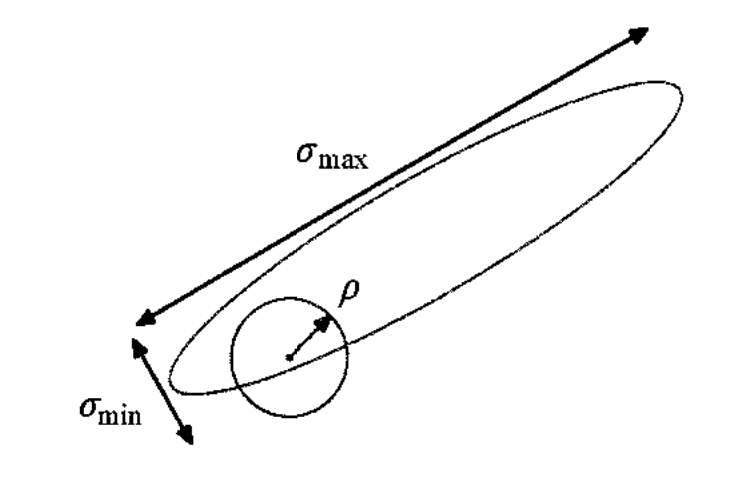
\includegraphics[width=0.42\textwidth]{ch14-fig14.10-mh-anisotropic.png}
\caption{使用各向同性的提议分布（蓝色圆圈）从相关多元 Gauss 分布（红色椭圆）中进行 Metropolis-Hastings 采样的示意图，后者在不同方向上具有完全不同的标准差。为了保持较低的拒绝率，提议分布的尺度 $\sigma$ 应该与最小标准差 $\sigma_{\min}$ 的数量级相当，这导致了随机游走行为，其中大致独立的状态之间分隔的步数是 $\left(\sigma_{\max}/\sigma_{\min}\right)^{2}$ 阶的，其中 $\sigma_{\max}$ 是最大的标准差}
\label{figure:ch14-各向同性提议}
\end{figure}

\subsection{Gibbs 采样}\label{subsection:ch14-gibbs采样}

Gibbs 采样（Geman and Geman, 1984）是一种简单且使用广泛的采样策略，可以看作 Metropolis-Hastings 算法的一个特例。考虑分布 $p(\bm{z})=p\!\left(z_{1},\cdots,z_{M}\right)$，我们希望从中采样，假设我们已经为 Markov 链选择了一些初始状态。Gibbs 采样过程中的每一步都包含用我们从一个变量的条件分布中抽取的值替换该变量的值，该条件分布是以其余变量的值为条件的。因此，可通过从分布 $p\!\left(z_{i}\mid\bm{z}_{\setminus i}\right)$ 中采样来替换 $z_{i}$，其中 $\bm{z}_{\setminus i}$ 表示 $\left\{z_{1},\cdots,z_{M}\right\}$ 但其中不包括 $z_{i}$，这个过程要么按某种特定顺序循环遍历变量，要么在每一步随机从某些分布中选择要更新的变量。

\begin{definition}[Gibbs 采样]\label{definition:ch14-gibbs采样}
设 $p(\bm{z})=p\!\left(z_{1},\cdots,z_{M}\right)$ 为目标分布，$\bm{z}^{(0)}$ 为初始状态。Gibbs 采样按如下方式迭代：在第 $\tau$ 步依次（或按某个次序）对每个分量 $i\in\{1,\cdots,M\}$，从条件分布
\begin{align*}
p\!\left(z_{i}\mid\bm{z}_{\setminus i}\right)=p\!\left(z_{i}\mid z_{1},\cdots,z_{i-1},z_{i+1},\cdots,z_{M}\right)
\end{align*}
中抽取新值替换 $z_{i}$，其余分量保持不变。
\end{definition}

% SUPPLEMENT: parent=definition:ch14-gibbs采样; kind=motivation; location=紧随其后的 remark（重构新增）
\begin{remark}（重构新增）Gibbs 采样的动机是「把联合采样化为一维条件采样」：直接从 $p(\bm{z})$ 采样困难，但从 $p\!\left(z_{i}\mid\bm{z}_{\setminus i}\right)$ 采样往往容易（例如在图模型中，$z_{i}$ 的条件分布只依赖其 Markov 毯，见\cref{figure:ch14-markov毯}）。它有两个前提：其一，所有条件分布都必须可以采样，若某个条件分布本身难以采样，Gibbs 就无法进行（可改用 Metropolis-Hastings 提议）；其二，条件分布必须在支撑集上无零概率区域，否则链被限制在状态空间的一部分、遍历性失效（见\cref{exercise:ch14-13}）。定义中「依次」与「随机选择」两种扫描方式都正确，因为它们分别对应\eqref{align:ch14-混合转移}与\eqref{align:ch14-复合转移}的转移核；实践中按固定次序扫描更常用，但随机扫描更容易保证可逆性。
\end{remark}

例如，假设我们有一个关于 $3$ 个变量的分布 $p\!\left(z_{1},z_{2},z_{3}\right)$，在时间步 $\tau$，我们选定了值 $z_{1}^{(\tau)}$、$z_{2}^{(\tau)}$ 和 $z_{3}^{(\tau)}$。首先将 $z_{1}^{(\tau)}$ 替换为通过从如下条件分布中采样获得的新值 $z_{1}^{(\tau+1)}$：
\begin{align}
p\!\left(z_{1}\mid z_{2}^{(\tau)},z_{3}^{(\tau)}\right).
\label{align:ch14-gibbs条件1}
\end{align}
然后将 $z_{2}^{(\tau)}$ 替换为通过从如下条件分布中采样获得的新值 $z_{2}^{(\tau+1)}$：
\begin{align}
p\!\left(z_{2}\mid z_{1}^{(\tau+1)},z_{3}^{(\tau)}\right).
\label{align:ch14-gibbs条件2}
\end{align}
这样新的 $z_{1}$ 值便可立即在后续的采样步骤中使用。用我们从如下条件分布中抽取的样本 $z_{3}^{(\tau+1)}$ 更新 $z_{3}^{(\tau)}$：
\begin{align}
p\!\left(z_{3}\mid z_{1}^{(\tau+1)},z_{2}^{(\tau+1)}\right).
\label{align:ch14-gibbs条件3}
\end{align}
以此类推，依次循环遍历这 $3$ 个变量。

\begin{quote}
\small
\textbf{算法 14.3：Gibbs 采样}\\
\textbf{输入：}初始值 $\left\{z_{i}:i\in\{1,\cdots,M\}\right\}$；条件分布 $\left\{p\!\left(z_{i}\mid\left\{z_{j}\right\}_{j\neq i}\right):i\in\{1,\cdots,M\}\right\}$；迭代次数 $T$。\\
\textbf{输出：}最终值 $\left\{z_{i}:i\in\{1,\cdots,M\}\right\}$。\\
对 $\tau\in\{1,\cdots,T\}$：\\
\quad 对 $i\in\{1,\cdots,M\}$：\\
\quad\quad 从 $p\!\left(z_{i}\mid\left\{z_{j}\right\}_{j\neq i}\right)$ 中采样 $z_{i}$；\\
返回 $\left\{z_{i}:i\in\{1,\cdots,M\}\right\}$。
\end{quote}

我们可以将 Gibbs 采样过程看作是 Metropolis-Hastings 算法的一个特定实例。考虑一个涉及变量 $z_{i}$ 的 Metropolis-Hastings 采样步骤，其余变量 $\bm{z}_{\setminus i}$ 保持不变，从 $\bm{z}$ 到 $\bm{z}^{\star}$ 的转移概率由 $q_{k}\!\left(\bm{z}^{\star}\mid\bm{z}\right)=p\!\left(z_{i}^{\star}\mid\bm{z}_{\setminus i}\right)$ 给出。注意 $\bm{z}_{\setminus i}^{\star}=\bm{z}_{\setminus i}$，因为这些分量在采样步骤中未发生改变。同样，$p(\bm{z})=p\!\left(z_{i}\mid\bm{z}_{\setminus i}\right)p\!\left(\bm{z}_{\setminus i}\right)$，因此，Metropolis-Hastings 算法\eqref{align:ch14-mh接受概率}中确定接受概率的因子由下式给出：
\begin{align}
A\!\left(\bm{z}^{\star},\bm{z}\right)&=\frac{p\!\left(\bm{z}^{\star}\right)q_{k}\!\left(\bm{z}\mid\bm{z}^{\star}\right)}{p(\bm{z})q_{k}\!\left(\bm{z}^{\star}\mid\bm{z}\right)}\nonumber\\
&=\frac{p\!\left(z_{i}^{\star}\mid\bm{z}_{\setminus i}^{\star}\right)p\!\left(\bm{z}_{\setminus i}^{\star}\right)p\!\left(z_{i}\mid\bm{z}_{\setminus i}^{\star}\right)}{p\!\left(z_{i}\mid\bm{z}_{\setminus i}\right)p\!\left(\bm{z}_{\setminus i}\right)p\!\left(z_{i}^{\star}\mid\bm{z}_{\setminus i}\right)}=1,
\label{align:ch14-gibbs接受率}
\end{align}
其中 $\bm{z}_{\setminus i}^{\star}=\bm{z}_{\setminus i}$。因此，Metropolis-Hastings 采样步骤总是可以接受。

\begin{proposition}[Gibbs 采样是 Metropolis-Hastings 的特例]\label{proposition:ch14-gibbs是mh特例}
以 $q_{k}\!\left(\bm{z}^{\star}\mid\bm{z}\right)=p\!\left(z_{i}^{\star}\mid\bm{z}_{\setminus i}\right)$ 为提议分布、其余分量保持不变的 Metropolis-Hastings 步骤，其接受概率恒为 $1$，即\eqref{align:ch14-gibbs接受率}成立。
\end{proposition}

\begin{proof}
因 $\bm{z}_{\setminus i}^{\star}=\bm{z}_{\setminus i}$，有 $p\!\left(\bm{z}_{\setminus i}^{\star}\right)=p\!\left(\bm{z}_{\setminus i}\right)$，且 $p\!\left(z_{i}\mid\bm{z}_{\setminus i}^{\star}\right)=p\!\left(z_{i}\mid\bm{z}_{\setminus i}\right)$、$p\!\left(z_{i}^{\star}\mid\bm{z}_{\setminus i}\right)=p\!\left(z_{i}^{\star}\mid\bm{z}_{\setminus i}^{\star}\right)$。把这些代入\eqref{align:ch14-mh接受概率}的比值，分子与分母逐项相同，故比值等于 $1$，接受概率 $\min\left(1,1\right)=1$。
\end{proof}

% SUPPLEMENT: parent=proposition:ch14-gibbs是mh特例; kind=motivation; location=紧随其后的 remark（重构新增）
\begin{remark}（重构新增）这一命题说明 Gibbs 采样「无需拒绝」：提议分布恰好是目标分布的一个条件分布，于是\eqref{align:ch14-gibbs接受率}中的四个因子两两相消。这带来两个好处：每一步都产生新样本（没有浪费），且不需要调节步长；代价是每个样本只改变一个分量，当分量之间高度相关时，链只能沿坐标方向移动，形成缓慢的锯齿状随机游走（见\cref{figure:ch14-gibbs采样}）。命题也说明了 Gibbs 的适用边界：只有当所有条件分布都能精确采样时，接受率才恒为 $1$；若用近似方法从条件分布采样，则必须退回 Metropolis-Hastings 并显式使用其接受率。
\end{remark}

为了证明该过程从目标分布中采样，我们首先注意到分布 $p(\bm{z})$ 是 Gibbs 采样步骤中的一个单独的不变量，因此它也是整个 Markov 链的不变量。这是因为当我们从 $p\!\left(z_{i}\mid\bm{z}_{\setminus i}\right)$ 中采样时，边缘分布 $p\!\left(\bm{z}_{\setminus i}\right)$ 显然是不变的，因为 $\bm{z}_{\setminus i}$ 的值没有发生改变。同样，定义的每一步采样都从正确的条件分布 $p\!\left(z_{i}\mid\bm{z}_{\setminus i}\right)$ 中采样。因为这些条件分布和边缘分布共同指定了联合分布，所以我们可以看到联合分布本身是不变的。

\begin{proposition}[Gibbs 采样的不变性]\label{proposition:ch14-gibbs不变性}
设 $p(\bm{z})>0$ 在状态空间上成立。则对每个分量 $i$，以 $p\!\left(z_{i}\mid\bm{z}_{\setminus i}\right)$ 为条件分布的 Gibbs 更新以 $p$ 为不变分布；从而整个 Gibbs 扫描（无论按固定次序还是随机次序）也以 $p$ 为不变分布。
\end{proposition}

\begin{proof}
记 $\bm{z}=\left(z_{i},\bm{z}_{\setminus i}\right)$。Gibbs 更新把 $z_{i}$ 换成 $z_{i}'\sim p\!\left(\cdot\mid\bm{z}_{\setminus i}\right)$，故更新后的联合密度为
\begin{align*}
p\!\left(z_{i}',\bm{z}_{\setminus i}\right)=p\!\left(z_{i}'\mid\bm{z}_{\setminus i}\right)p\!\left(\bm{z}_{\setminus i}\right)=p\!\left(z_{i}',\bm{z}_{\setminus i}\right),
\end{align*}
即 $p$ 不变。若按固定次序依次更新全部分量，则每一步都不变 $p$，复合后仍不变 $p$；若随机挑选分量，则由\cref{proposition:ch14-混合转移不变}，混合后的转移核也不变 $p$。
\end{proof}

% SUPPLEMENT: parent=proposition:ch14-gibbs不变性; kind=motivation; location=紧随其后的 remark（重构新增）
\begin{remark}（重构新增）证明的关键是「条件分布乘边缘分布等于联合分布」：Gibbs 更新只重新抽取 $z_{i}$，而新值恰好来自联合分布关于 $z_{i}$ 的条件，因此更新后的联合密度与原联合密度逐点相等——这比 Metropolis-Hastings 的「流量相等」更强，是逐点的等式。条件 $p(\bm{z})>0$ 保证所有条件分布有定义（否则 $p\!\left(z_{i}\mid\bm{z}_{\setminus i}\right)$ 可能分母为零）。注意这里论证的是\emph{不变性}而非遍历性：若状态空间被零概率区域分割，不变性仍成立但链可能只在其中一个连通块内游走。
\end{remark}

为了完整地描述该算法，还需要指定初始状态的分布，尽管在多次迭代后抽取的样本实际上独立于此分布。当然，从 Markov 链中连续抽取的样本将高度相关，因此要获得几乎独立的样本，就需要对序列进行子样本采样。

确保能从正确分布中进行 Gibbs 采样的第二个条件是要具有遍历性（ergodic）。具有遍历性的一个充分条件是条件分布不存在零概率区域。如果是这种情况，那么 $\bm{z}$ 空间中的任意一点都可以通过有限步骤到达其他任意一点，每一步都包括更新每个分量变量中的一个。如果不满足这个要求，即某些条件分布存在零概率区域，那么遍历性（如果适用）必须被显式地证明。

与 Metropolis 算法类似，我们可以通过研究 Gibbs 采样在特定分布（例如 Gauss 分布）上的应用来深入了解其行为。考虑\cref{figure:ch14-gibbs采样}所示的两个变量中相关 Gauss 分布，其条件分布的宽度为 $l$，边缘分布的宽度为 $L$。典型的步长由条件分布决定，并且将是 $l$ 阶的。由于状态根据随机游走演化，因此为了获得来自分布的独立样本，所需的步数将是 $\left(L/l\right)^{2}$ 阶的。当然，如果 Gauss 分布是不相关的，那么 Gibbs 采样过程将是最优的。对于这个简单问题，我们可以旋转坐标系，使得新变量不相关。但是，在实际应用中，我们通常不可能找到这样的转换。

\begin{figure}[htbp]
\centering
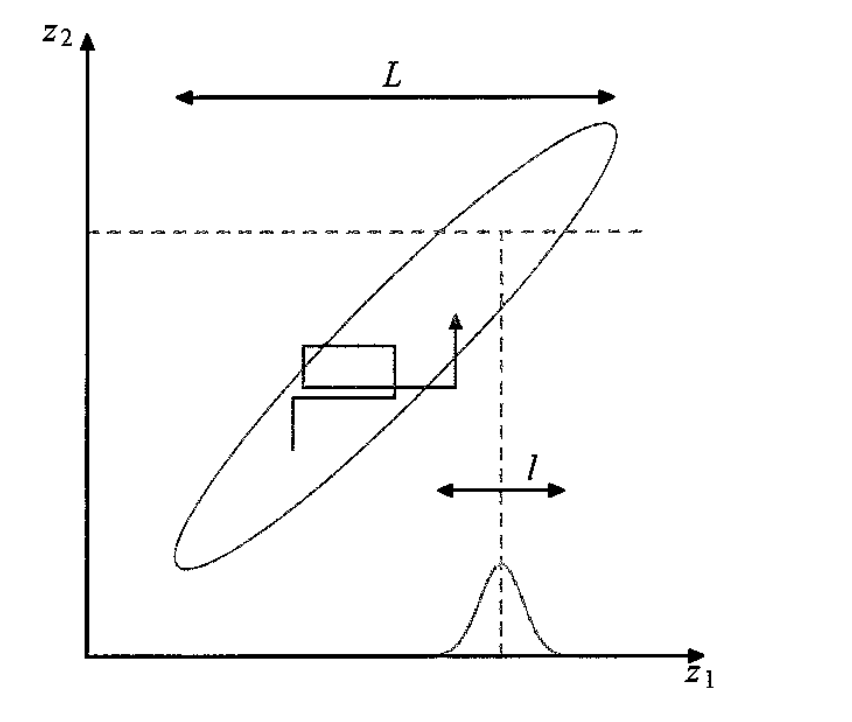
\includegraphics[width=0.48\textwidth]{ch14-fig14.11-gibbs.png}
\caption{交替更新两个变量的 Gibbs 采样示意图，这两个变量的分布是相关 Gauss 分布。步长由条件分布（绿色曲线）的标准差控制，为 $\mathcal{O}(l)$，这导致在联合分布（红色椭圆）拉长方向上的进展缓慢。从分布中获得一个独立样本所需的步数是 $\mathcal{O}\left(\left(L/l\right)^{2}\right)$}
\label{figure:ch14-gibbs采样}
\end{figure}

由于基本的 Gibbs 采样技术一次只考虑一个变量，因此连续样本之间存在强依赖关系。在另一种极端情况下，如果我们能够直接从联合分布中采样（实际上这种操作很难实现），则连续样本将是独立的。我们可以采用一种折中策略来改进简单的 Gibbs 采样，即连续地从变量组而不是单个变量中采样。这可以通过分块 Gibbs（blocking Gibbs）采样算法实现，该算法选择变量块（不一定是互斥的），然后依次对每个块中的变量进行联合采样，条件是其他所有变量保持其当前值（Jensen, Kong, and Kjaerulff, 1995）。

减少 Gibbs 采样中随机游走行为的一种方法称为超松弛（over-relaxation）（Adler, 1981）。在它的原始形式中，它适用于条件分布是 Gauss 分布的问题，就是说，「条件分布为 Gauss 分布」所涵盖的分布类型比「多元 Gauss 分布」更广泛。例如，非 Gauss 分布 $p(z,y)\propto\exp\left(-z^{2}y^{2}\right)$ 具有条件 Gauss 分布。在 Gibbs 采样的每一步，特定分量 $z_{i}$ 具有均值为 $\mu_{i}$、方差为 $\sigma_{i}^{2}$ 的条件分布。在超松弛框架中，$z_{i}$ 的值被替换为
\begin{align}
z_{i}'=\mu_{i}+\alpha_{i}\left(z_{i}-\mu_{i}\right)+\sigma_{i}\left(1-\alpha_{i}^{2}\right)^{1/2}v,
\label{align:ch14-超松弛}
\end{align}
其中 $v$ 是一个有零均值和单位方差的 Gauss 随机变量，$\alpha$ 是一个参数，满足 $-1<\alpha<1$。当 $\alpha=0$ 时，该方法等同于标准的 Gibbs 采样；当 $\alpha<0$ 时，该步骤偏向于均值的相反侧。这一步骤保持了目标分布的不变性，因为如果 $z_{i}$ 有均值 $\mu_{i}$ 和方差 $\sigma_{i}^{2}$，那么 $z_{i}'$ 也将如此（见\cref{exercise:ch14-14}）。超松弛的作用是在变量高度相关时，鼓励状态空间中的定向运动。有序超松弛框架（ordered over-relaxation）（Neal, 1999）将这种方法推广到了非 Gauss 分布。

\begin{proposition}[超松弛更新保持条件分布]\label{proposition:ch14-超松弛不变}
设给定其余分量时 $z_{i}$ 的条件分布为 $\mathcal{N}\!\left(\mu_{i},\sigma_{i}^{2}\right)$，$v\sim\mathcal{N}(0,1)$ 且与 $z_{i}$ 独立，$\left|\alpha_{i}\right|<1$，$z_{i}'$ 由\eqref{align:ch14-超松弛}定义。则 $z_{i}'$ 的条件分布仍为 $\mathcal{N}\!\left(\mu_{i},\sigma_{i}^{2}\right)$。
\end{proposition}

\begin{proof}
记 $\xi=z_{i}-\mu_{i}$，则 $\xi\sim\mathcal{N}\!\left(0,\sigma_{i}^{2}\right)$。由\eqref{align:ch14-超松弛}，
\begin{align*}
z_{i}'-\mu_{i}=\alpha_{i}\xi+\sigma_{i}\left(1-\alpha_{i}^{2}\right)^{1/2}v.
\end{align*}
由独立性，$\mathbb{E}\left[z_{i}'-\mu_{i}\right]=\alpha_{i}\cdot0+0=0$，且
\begin{align*}
\operatorname{var}\left[z_{i}'\right]=\alpha_{i}^{2}\sigma_{i}^{2}+\sigma_{i}^{2}\left(1-\alpha_{i}^{2}\right)=\sigma_{i}^{2}.
\end{align*}
两个独立 Gauss 变量的线性组合仍为 Gauss 变量，故 $z_{i}'\sim\mathcal{N}\!\left(\mu_{i},\sigma_{i}^{2}\right)$。
\end{proof}

% SUPPLEMENT: parent=proposition:ch14-超松弛不变; kind=motivation; location=紧随其后的 remark（重构新增）
\begin{remark}（重构新增）超松弛的技巧是「保留均值与方差、但把新值推到均值的另一侧」：$\alpha<0$ 时 $z_{i}'-\mu_{i}$ 与 $z_{i}-\mu_{i}$ 反号，于是链不再沿坐标方向做小步随机游走，而是跨过均值继续前进，从而削弱相邻样本的相关性。条件 $\left|\alpha_{i}\right|<1$ 保证 $\left(1-\alpha_{i}^{2}\right)^{1/2}$ 为实数且方差为正；$\alpha=1$ 时更新退化为 $z_{i}'=\mu_{i}+z_{i}-\mu_{i}=z_{i}$（不动），$\alpha=-1$ 时退化为关于均值的镜像反射。命题只说明了\emph{条件分布}不变，由于 Gibbs 的每一步都是条件更新，这与联合分布不变等价（见\cref{proposition:ch14-gibbs不变性}）。注意该方法要求条件分布为 Gauss 且能算出 $\mu_{i},\sigma_{i}^{2}$，对一般分布需改用有序超松弛。
\end{remark}

Gibbs 采样的实用性取决于从条件分布 $p\!\left(z_{i}\mid\bm{z}_{\setminus i}\right)$ 中采样的难度。对于使用有向图模型表示的概率分布，单个节点的条件分布仅依赖于相应 Markov 毯中的变量，如\cref{figure:ch14-markov毯}所示。对于有向图，各个节点的基于其父节点的条件分布的广泛选择将导致 Gibbs 采样的条件分布是对数凹的。因此，\cref{subsection:ch14-适应性拒绝采样}讨论的自适应拒绝采样方法为从有向图中进行 Monte Carlo 采样提供了一个具有广泛适用性的框架。

\begin{figure}[htbp]
\centering
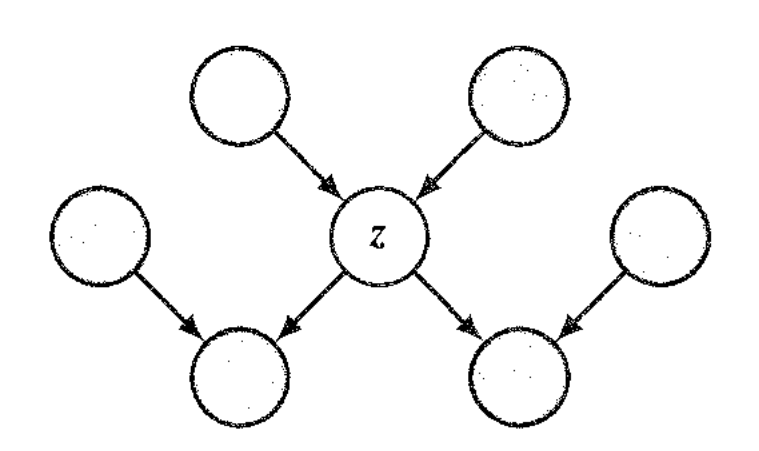
\includegraphics[width=0.32\textwidth]{ch14-fig14.12-markov-blanket.png}
\caption{Gibbs 采样需要从一个变量 $z$ 的条件分布中抽取样本，该条件分布是基于其余变量的。对于有向图模型，这个条件分布只是 Markov 毯中节点状态的函数，Markov 毯在图中以蓝色阴影显示，它包括了父节点、子节点以及共同父节点}
\label{figure:ch14-markov毯}
\end{figure}

\begin{definition}[Markov 毯]\label{definition:ch14-markov毯}
在有向图模型中，节点 $i$ 的 Markov 毯（Markov blanket）由 $i$ 的父节点、子节点以及子节点的其他父节点组成。给定 Markov 毯中所有变量的取值，$z_{i}$ 与图中其余变量条件独立，即 $p\!\left(z_{i}\mid\bm{z}_{\setminus i}\right)=p\!\left(z_{i}\mid\mathrm{mb}(i)\right)$，其中 $\mathrm{mb}(i)$ 表示 Markov 毯中的变量集合。
\end{definition}

% SUPPLEMENT: parent=definition:ch14-markov毯; kind=motivation; location=紧随其后的 remark（重构新增）
\begin{remark}（重构新增）Markov 毯把「计算条件分布需要哪些变量」这一全局问题化为局部问题：对 Gibbs 采样而言，更新 $z_{i}$ 时只需知道其 Markov 毯的取值，而不必访问整张图，这使得高维图模型上的 Gibbs 采样在计算上可行。毯中之所以还要包含「子节点的其他父节点」，是因为这些变量与 $z_{i}$ 通过共同子节点产生依赖（解释消除效应）；若漏掉它们，条件分布会被错误地简化。对无向图模型，Markov 毯就是与节点相邻的所有节点，这一差别源于有向图与无向图的因子分解方式不同。\cref{figure:ch14-markov毯}中的蓝色阴影即示意这一集合。
\end{remark}

\subsection{祖先采样}\label{subsection:ch14-祖先采样}

对于许多模型来说，联合分布 $p(\bm{z})$ 可以方便地用图模型的术语来表示。对于一个没有观测变量的有向图，可以直接使用祖先采样（ancestral sampling）方法从联合分布中采样。联合分布由下式指定：
\begin{align}
p(\bm{z})=\prod_{i=1}^{M}p\!\left(\bm{z}_{i}\mid\mathrm{pa}(i)\right),
\label{align:ch14-祖先采样分解}
\end{align}
其中 $\bm{z}_{i}$ 是与节点 $i$ 关联的一组变量，$\mathrm{pa}(i)$ 表示与节点 $i$ 的父节点关联的一组变量。

\begin{definition}[祖先采样]\label{definition:ch14-祖先采样}
设联合分布具有\eqref{align:ch14-祖先采样分解}的因子分解形式。按拓扑序 $z_{1},\cdots,z_{M}$ 遍历各节点，依次从条件分布 $p\!\left(\bm{z}_{i}\mid\mathrm{pa}(i)\right)$ 中抽取样本，则得到的 $\left(\bm{z}_{1},\cdots,\bm{z}_{M}\right)$ 是联合分布 $p(\bm{z})$ 的一个样本。这一方法称为祖先采样（ancestral sampling）。
\end{definition}

% SUPPLEMENT: parent=definition:ch14-祖先采样; kind=motivation; location=紧随其后的 remark（重构新增）
\begin{remark}（重构新增）祖先采样之所以正确，是因为拓扑序保证每一步的所有父变量都已被实例化，条件分布 $p\!\left(\bm{z}_{i}\mid\mathrm{pa}(i)\right)$ 因而总是有定义的；把各步抽样的条件密度相乘，恰好得到\eqref{align:ch14-祖先采样分解}，即联合分布。它要求每一步都能从条件分布中采样，并且图中没有观测变量；一旦存在证据（被观测的节点），条件分布就变成后验分布，祖先采样不能直接使用，必须引入重要性加权（见下文似然加权采样）。祖先采样的计算代价是 $O(M)$ 次条件采样，是图模型中最快的精确采样方法，但它只适用于有向无环图。
\end{remark}

为了获得联合分布的一个样本，我们按照 $z_{1},\cdots,z_{M}$ 的顺序遍历这组变量，并从条件分布 $p\!\left(\bm{z}_{i}\mid\mathrm{pa}(i)\right)$ 中采样。这总是可能的，因为在每个步骤，所有父变量都会被实例化。遍历图一次后，我们将获得联合分布的一个样本。这里假设我们可以从每个节点的各条件分布中采样。

考虑这样一个有向图，其部分节点组成了证据集 $\varepsilon$，并被观测值实例化过。原则上可以扩展上述过程，至少对于代表离散变量的节点，我们可以给出以下逻辑采样方法（Henrion, 1988），它可以看作重要性采样的一种特殊情况（见\cref{subsection:ch14-重要性采样}）。在每一步，当为一个观测值已知的变量 $z_{i}$ 获得一个采样值时，对采样值与观测值进行比较：如果它们一致，则保留采样值，并继续依次处理下一个变量；然而，如果它们不一致，则丢弃到目前为止的整个样本，重新从图的第一个节点开始。这种算法可以正确地从后验分布中采样，因为它仅仅相当于从隐变量和数据变量的联合分布中抽取样本，然后丢弃那些与观测数据不一致的样本（在发现一个不一致的值后就不再从联合分布中继续采样，从而稍微提高了效率）。然而，随着观测变量数量的增加和这些变量可以取的状态数量的增加，从后验分布中接受一个样本的整体概率迅速降低，因此这种方法在实践中很少使用。

这种方法的改进版称为似然加权采样（likelihood weighted sampling）（Fung and Chang, 1990; Shachter and Peot, 1990），它基于祖先采样并结合了重要性采样。对于每一个变量，如果该变量在证据集中，那么把它设置为其实例化的值。如果它不在证据集中，则从条件分布 $p\!\left(z_{i}\mid\mathrm{pa}(i)\right)$ 中采样，其中条件变量设置为其当前采样的值。随后产生的样本 $\bm{z}$ 的权重由下式给出（见\cref{exercise:ch14-15}）：
\begin{align}
r(\bm{z})=\prod_{z_{i}\notin\varepsilon}\frac{p\!\left(z_{i}\mid\mathrm{pa}(i)\right)}{p\!\left(z_{i}\mid\mathrm{pa}(i)\right)}\prod_{z_{i}\in\varepsilon}\frac{p\!\left(z_{i}\mid\mathrm{pa}(i)\right)}{1}=\prod_{z_{i}\in\varepsilon}p\!\left(z_{i}\mid\mathrm{pa}(i)\right).
\label{align:ch14-似然加权权重}
\end{align}

\begin{definition}[似然加权采样]\label{definition:ch14-似然加权采样}
给定有向图模型、证据集 $\varepsilon$ 与观测值 $\hat{z}_{i}$（$i\in\varepsilon$）。似然加权采样按拓扑序处理各节点：若 $z_{i}\in\varepsilon$，则令 $z_{i}=\hat{z}_{i}$；否则从 $p\!\left(z_{i}\mid\mathrm{pa}(i)\right)$ 中采样。最终样本 $\bm{z}$ 附带权重\eqref{align:ch14-似然加权权重}。
\end{definition}

% SUPPLEMENT: parent=definition:ch14-似然加权采样; kind=motivation; location=紧随其后的 remark（重构新增）
\begin{remark}（重构新增）似然加权的动机是「不丢弃任何样本」：逻辑采样在证据与采样值不一致时整条样本作废，接受率随证据变量个数与状态数指数下降；似然加权则把证据节点固定为观测值、把它本应出现的先验概率记入权重，于是每条样本都被保留，权重承担了「这条样本在证据下的合理性」。它本质上是重要性采样，提议分布取为「先验 + 证据上的 delta」，目标分布取为后验。使用条件有三：其一，必须能从每个非证据节点的先验条件分布 $p\!\left(z_{i}\mid\mathrm{pa}(i)\right)$ 中采样，这与祖先采样相同；其二，对后验支撑上的任意取值都应有 $p\!\left(z_{i}\mid\mathrm{pa}(i)\right)>0$，否则权重为零或未定义，后验的相应区域被系统性漏掉；其三，权重只依赖证据节点，因此其方差通常远小于逻辑采样的接受率倒数。当证据很多且每条证据的概率都很小时，权重会高度集中，有效样本量下降，这是似然加权的主要局限。\end{remark}

\begin{proposition}[似然加权采样的权重]\label{proposition:ch14-似然加权权重}
在\cref{definition:ch14-似然加权采样}的设定下，若 $q(\bm{z})$ 表示该采样过程产生的分布，则后验分布 $p\!\left(\bm{z}\mid\varepsilon\right)$ 关于 $q$ 的重要性权重为\eqref{align:ch14-似然加权权重}，即
\begin{align*}
\frac{p\!\left(\bm{z}\mid\varepsilon\right)}{q(\bm{z})}\propto\prod_{z_{i}\in\varepsilon}p\!\left(z_{i}\mid\mathrm{pa}(i)\right).
\end{align*}
\end{proposition}

\begin{proof}
采样过程对非证据节点按先验抽样、对证据节点取固定值，故
\begin{align*}
q(\bm{z})=\prod_{z_{i}\notin\varepsilon}p\!\left(z_{i}\mid\mathrm{pa}(i)\right)\prod_{z_{i}\in\varepsilon}\delta\!\left(z_{i}-\hat{z}_{i}\right).
\end{align*}
另一方面，由\eqref{align:ch14-祖先采样分解}，联合分布为 $p(\bm{z})=\prod_{i}p\!\left(z_{i}\mid\mathrm{pa}(i)\right)$，而后验分布 $p\!\left(\bm{z}\mid\varepsilon\right)=p(\bm{z})\mathbb{I}\left(\bm{z}_{\varepsilon}=\hat{\bm{z}}_{\varepsilon}\right)/p(\varepsilon)$ 与 $p(\bm{z})\mathbb{I}\left(\bm{z}_{\varepsilon}=\hat{\bm{z}}_{\varepsilon}\right)$ 成比例。于是
\begin{align*}
\frac{p\!\left(\bm{z}\mid\varepsilon\right)}{q(\bm{z})}\propto\frac{\prod_{z_{i}\notin\varepsilon}p\!\left(z_{i}\mid\mathrm{pa}(i)\right)\prod_{z_{i}\in\varepsilon}p\!\left(\hat{z}_{i}\mid\mathrm{pa}(i)\right)}{\prod_{z_{i}\notin\varepsilon}p\!\left(z_{i}\mid\mathrm{pa}(i)\right)\prod_{z_{i}\in\varepsilon}\delta\!\left(z_{i}-\hat{z}_{i}\right)},
\end{align*}
在 $\bm{z}_{\varepsilon}=\hat{\bm{z}}_{\varepsilon}$ 上两个 $\delta$ 因子相消，非证据节点的因子相消，剩下的正是 $\prod_{z_{i}\in\varepsilon}p\!\left(\hat{z}_{i}\mid\mathrm{pa}(i)\right)$，即\eqref{align:ch14-似然加权权重}。
\end{proof}

% SUPPLEMENT: parent=proposition:ch14-似然加权权重; kind=motivation; location=紧随其后的 remark（重构新增）
\begin{remark}（重构新增）似然加权采样的意思是「照常按先验采样，但把证据节点的采样概率记在权重里」：证据节点不再被采样，而是被固定，于是它们的先验概率不再出现在样本分布 $q$ 中，却仍是后验分布的一部分，权重正好补上这一缺口。与逻辑采样相比，它不会因为证据与采样值不一致而丢弃整条样本，因此效率高得多；代价是权重可能很小（当证据在模型下概率很低时），有效样本量随之下降。命题中的 $\delta$ 记号是连续情形下的形式写法，离散情形应理解为指示函数 $\mathbb{I}\left(z_{i}=\hat{z}_{i}\right)$；无论哪种情形，结论都成立。这一权重形式与\cref{subsection:ch14-重要性采样}的重要性权重完全一致，只是在图模型上被因式分解了。
\end{remark}

这种方法可以进一步使用自重要性采样（self-importance sampling）（Shachter and Peot, 1990）扩展，其中重要性采样分布不断更新，以反映当前估计的后验分布。

\end{document}
